\documentclass[a4paper, 12pt]{article}
%\usepackage[T1]{fontenc}
\usepackage[left=2cm,right=2cm,top=2cm,bottom=2cm,includeheadfoot]{geometry}
\usepackage[utf8]{inputenc}
\usepackage[ngerman]{babel}
\usepackage{enumitem}
\usepackage{pdfpages}
\usepackage{ulem} 
\usepackage{graphicx}
\usepackage{caption}
\usepackage{subcaption}
\usepackage{listings}
\usepackage{verbatim}
\usepackage{fancyhdr}
\usepackage{hyperref}
\lstset{
<<<<<<< HEAD
	language=Java,
=======
	language=java,
>>>>>>> c1585b9eb1d3da72108067a08438cf1b411f54d8
	extendedchars=\true,
	inputencoding=utf8,
	stringstyle=\ttfamily\small, 
	showstringspaces=false,
	commentstyle=\color{codegreen},
	keywordstyle=\color{blue},
	stringstyle=\color{codegray}, 
	basicstyle=\ttfamily\small,
	breakatwhitespace=false,         
	breaklines=true, 
	captionpos=b,                    
	keepspaces=true,                 
	numbers=left,                    
	numbersep=5pt,                  
	showspaces=false,                
	showstringspaces=false,
	showtabs=false,                  
	tabsize=2,
	aboveskip=1em,
}
\usepackage{color}
\usepackage{comment}


\definecolor{codegreen}{rgb}{0,0.6,0}
\definecolor{codegray}{rgb}{0.5,0.5,0.5}
%\definecolor{backcolour}{rgb}{0.95,0.95,0.92}

\lstset{language=Java}

\pagestyle{fancy}
\lhead[Sascha Beyer, David Schneebauer]{Sascha Beyer, David Schneebauer}
\chead[Projektarbeit Hurace]{Projektarbeit Hurace}
\rhead[SWK5 GRP1 SEBakk BB WS18-19]{SWK5 GRP1 SEBakk BB WS18-19}

%opening
\title{Projektarbeit Hurace}
\author{Sascha Beyer, David Schneebauer}
\date{\today{}, Hagenberg}

\begin{document}
	\maketitle
	\tableofcontents
	\newpage
	\section{Ausbaustufe 1}
	\subsubsection{Datenbankmodell}

	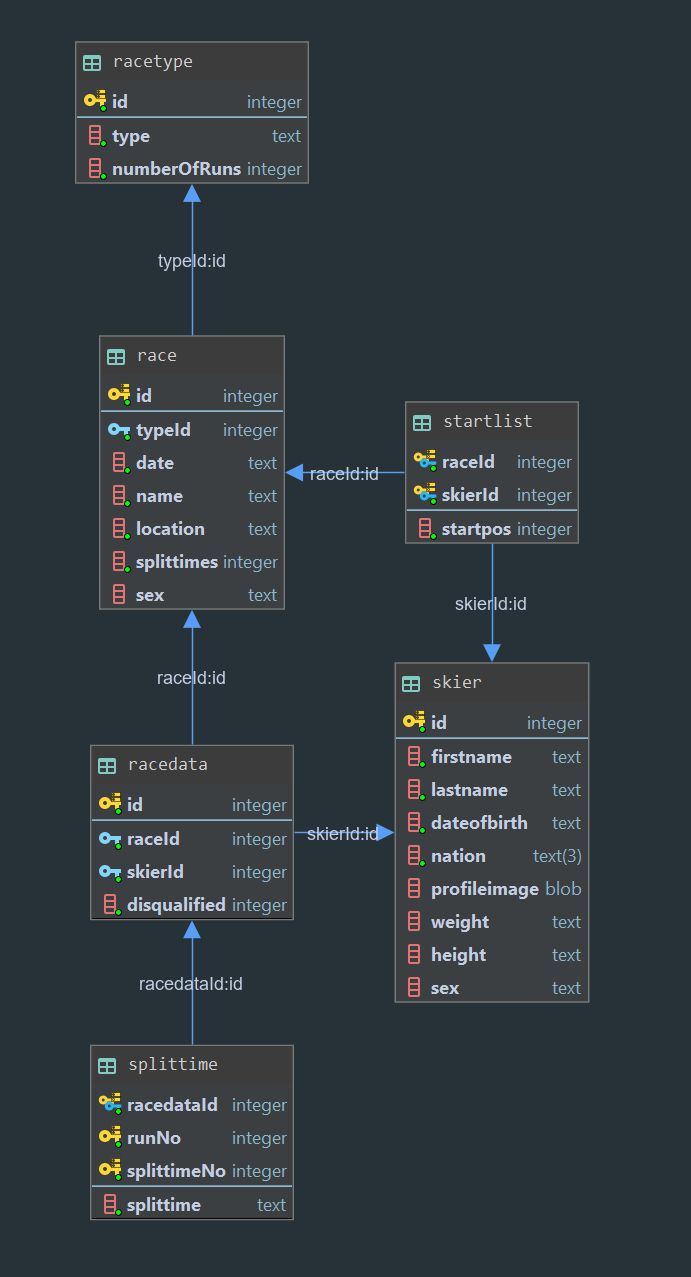
\includegraphics[width=.7\textwidth]{img/huraceDB.png}
	%\lstinputlisting[language=Java]{../Dal/Interface/IRaceDao.cs}
	%\newpage
	%\lstinputlisting[language=Java]{../src/queues/DHeapQueue.java}
	%\newpage
	\newpage
	\subsubsection{Datenbankzugriffsschicht}
	
	Zur persistierung der Daten wird eine SQLite Datenbank verwendet.
	Für jede Entität sind Dao Klassen implementiert. Diese stellen Methoden für Operationen auf der Datenbank zur Verfügung. Zur Herstellung der Verbindung wird das Factory Pattern verwendet. Über eine Konfigurationsdatei werden Informationen zum Datenbanktyp zur Verfügung gestellt.
	 
	%\includegraphics[width=.8\textwidth]{img/main_1.png}
	%\\
	%\includegraphics[width=.8\textwidth]{img/main_2.png}
	%\\
	%\includegraphics[width=.8\textwidth]{img/main_3.png}
	\textbf{IRaceDao}
	\lstinputlisting[language=csh]{../Dal/Interface/IRaceDao.cs}
	\textbf{IRaceDataDao}
	\lstinputlisting[language=csh]{../Dal/Interface/IRaceDataDao.cs}
	\textbf{IRaceTypeDao}
	\lstinputlisting[language=csh]{../Dal/Interface/IRaceTypeDao.cs}
	\textbf{ISkierDao}
	\lstinputlisting[language=csh]{../Dal/Interface/ISkierDao.cs}
	\textbf{ISplittimeDao}
	\lstinputlisting[language=csh]{../Dal/Interface/ISplittimeDao.cs}
	\textbf{IStartListDao}
	\lstinputlisting[language=csh]{../Dal/Interface/IStartListDao.cs}
	
	

	\newpage	
\end{document}